\input{wg21common}

% Footnotes at bottom of page:
 \usepackage[bottom]{footmisc} 

% Table going across a page: 
 \usepackage{longtable}

 % Start sections at 0
% \setcounter{section}{-1}

% color boxes
\usepackage{tikz,lipsum,lmodern}
\usepackage[most]{tcolorbox}

%%%%%%%%%%%%%%%%%%%%%%%%%%%%%%%%%%%%%%%%%%%%%%%%

%TABLE OF CONTENTS SETTINGS

\usepackage{titlesec}
\usepackage{tocloft}

% Custom ToC layout because the default sucks
\cftsetindents{section}{0in}{0.24in}
\cftsetindents{subsection}{0.24in}{0.34in}
\cftsetindents{subsubsection}{0.58in}{0.44in}

% Needed later to reduce the ToC depth mid document
\newcommand{\changelocaltocdepth}[1]{%
  \addtocontents{toc}{\protect\setcounter{tocdepth}{#1}}%
  \setcounter{tocdepth}{#1}%
}

\setcounter{tocdepth}{3}

%%%%%%%%%%%%%%%%%%%%%%%%%%%%%%%%%%%%%%%%%%%%%%%%

\begin{document}
\title{Undefined and erroneous behaviour is a contract violation}
\author{ Timur Doumler \small(\href{mailto:papers@timur.audio}{papers@timur.audio})  \\
Ga\v sper A\v zman \small(\href{mailto:gasper.azman@gmail.com}{gasper.azman@gmail.com})   \\
Joshua Berne \small(\href{mailto:jberne4@bloomberg.net}{jberne4@bloomberg.net})  
}
\date{}
\maketitle

\begin{tabular}{ll}
Document \#: & P3100R1 \\
Date: &2024-10-16 \\
Project: & Programming Language C++ \\
Audience: & EWG, SG21, SG23
\end{tabular}

\begin{abstract}
In this paper, we propose to apply the semantics of Contracts \cite{P2900R8} to undefined behaviour in C++. By respecifying evaluations of core language constructs that would have undefined behaviour as \emph{contract violations}, we allow them to be checked, observed, enforced, and handled via a user-defined contract-violation handler, just like violations of user-authored contract assertions. We thus add a powerful and flexible new tool for improving the safety of C++. We also create a framework for reasoning, within the C++ Standard, about sanitisers and other existing strategies for mitigating undefined behaviour during program execution. Our proposed specification supersedes the concept of \emph{erroneous behaviour} introduced by \cite{P2795R5}.
\end{abstract}

%%%%%%%%%%%%%%%%%%%%%%%%%%%%%%%%%%%%%%%%%%%%%

\tableofcontents*
\pagebreak

%\section*{Revision history}

%Revision 0 (2024-04-16)
%\begin{itemize}
%\item Original version
%\end{itemize}

%\pagebreak

%%%%%%%%%%%%%%%%%%%%%%%%%%%%%%%%%%%%%%%%%%%%%

\section{Introduction}
\label{intro}

Improving safety and security is arguably the most important challenge for the future evolution of the C++ language (\cite{Bastien2023}). Governments and regulatory bodies have called for the tech industry to move away from C and C++ and towards \emph{safe} languages (\cite{NSA2022}, \cite{CR2023}, \cite{CISA2023}). Rust is a frequently cited example of a language that is considered \emph{safe}.

According to the definition in \cite{Carruth2023}, safety is characterised by invariants or limits on program behaviour in the face of bugs; safety bugs are bugs where some aspect of program behaviour has no invariants or limits. According to the definition of \cite{Abrahams2023}, a safe operation is one that cannot cause undefined behaviour; a safe language has only safe operations.

With the above definitions, C++ is not a safe language: both the core language and the C++ standard library allow for a multitude of ways in which a well-formed C++ can exhibit \emph{unbounded} undefined behaviour, that is, situations in which the C++ standard places no restrictions on the behaviour of the program. Bugs that trigger such unbounded undefined behaviour cause stability issues and can be exploited by threat actors, thereby causing security vulnerabilities. Among the most popular programming languages, the presence of unbounded undefined behaviour is a unique trait of C and C++. 

Realistically, we do not believe that it is possible to evolve C++ into a fully safe language under the above definition --- i.e., a language with no unbounded undefined behaviour --- in the foreseeable future (\cite{Doumler2023}). However, we can and should do what we can to significantly \emph{reduce} the amount of undefined behaviour in C++ programs, including in legacy code that may be recompiled but not modified on the source level.

Many ways to detect and mitigate undefined behaviour in C++ exist today. They range from engineering practices such as code reviews, coding guidelines, and meticulous coverage with unit tests to specialised tooling such as static analysers and sanitisers. However, while the use of such tools is usually strongly encouraged, they are not part of the core language and are therefore opt-in rather than opt-out. This is a major weakness of C++. For this reason, it is of particular importance to devote special attention to efforts to remove undefined behaviour from C++ on the language specification level.

These efforts are ongoing. For C++23, a common cause of undefined behaviour in range-based \tcode{for} loops has been removed (\cite{P2012R2}). For C++26, it will no longer be undefined behaviour to read an uninitialised value (\cite{P2795R5}) and to execute a trivial infinite loop (\cite{P2809R3}). Efforts to tackle the issue at a larger scale include the current work on safety profiles (\cite{P3274R0}) and adding a Rust-like borrow checker to C++ (\cite{P3390R0}). Outside of the C++ Standard committee, work in this space is being done by compiler vendors, for example the hardening modes in libc++\footnote{See \href{https://libcxx.llvm.org/Hardening.html}{https://libcxx.llvm.org/Hardening.html}.} and \tcode{-fbounds-safety} in Clang\footnote{See \href{https://clang.llvm.org/docs/BoundsSafety.html}{https://clang.llvm.org/docs/BoundsSafety.html}.}.

In \cite{P2900R8}, a Contracts facility is being proposed for inclusion in C++. One of the explicit goals of this proposal is to make C++ a safer language, and to make C++ programs more safe. The proposal has triggered discussions about whether this goal is being met, some going as far as saying that Contracts are not a safety feature at all: after all, they do not add new language guarantees, and instead focus on correctness checks during program evaluation, with no such checks being performed unless the developer adds explicit contract assertions to their code.

The goal of this paper is twofold: first, to explain how Contracts fit into the picture of making C++ more safe; second, to propose a design direction to make the Contracts facility more effective at detecting and mitigating undefined behaviour in C++, including in code that has no explicit contract annotations at all.

\section{The role of Contracts for Safe C++}
\label{role}

There are two possible approaches for removing occurrences of undefined behaviour from C++:
\begin{enumerate}
\item Reject the offending constructs at compile time;
\item Give the offending constructs well-defined behaviour during program execution.
\end{enumerate}
In general, approach 1 seems preferable, as it allows the developer to recognise and remove offending constructs earlier in the release cycle and the bug never makes it into the codebase.

However, not all undefined behaviour can be addressed with Approach 1. We can classify occurrences of undefined behaviour into two buckets: one for occurrences for which approach 1 seems feasible, and one for occurrences that can only be addressed by Approach 2 (see Figure~\ref{fig_buckets}).

%~~~~~~~~~~~~~~~~~~~~~~~~~~~~~~~~~~~~~~~~~~~~~~~~~~~~~~~~~~~~~~~~~~~
\begin{figure}[b]
\begin{center}
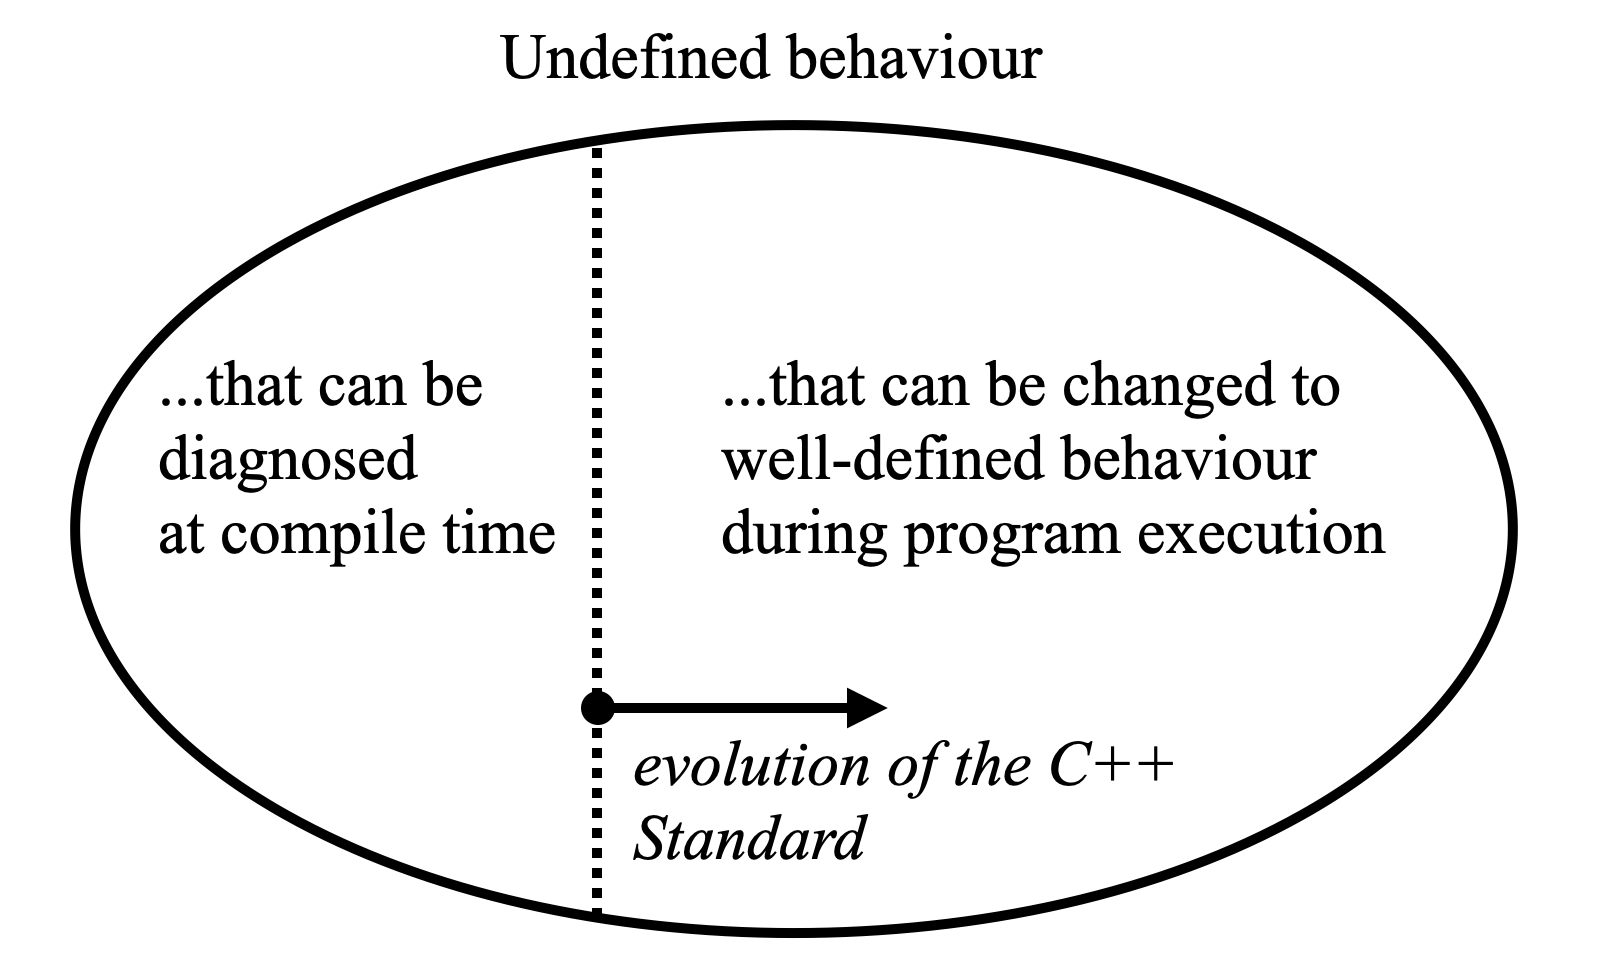
\includegraphics[scale=0.29]{images/p3100_buckets.png}
\end{center}
\caption{Two different approaches for removing occurrences of undefined behaviour from C++.}
\label{fig_buckets}
\end{figure}
%~~~~~~~~~~~~~~~~~~~~~~~~~~~~~~~~~~~~~~~~~~~~~~~~~~~~~~~~~~~~~~~~~~~

The boundary between these two buckets can be moved towards the right (i.e., by making more undefined behaviour being rejected at compile time) by evolving the C++ Standard towards introducing more constraints on well-formed constructs. This direction, however, is not viable in all cases.

In some cases, the reason why Approach 1 may not be viable is due to the existence of legacy code that needs to keep compiling and working as intended. Rejecting certain constructs could lead to an unacceptable amount of false positives that would break such code; for example, if we were to make it ill-formed to not initialise a variable, or to flow off the end of a non-\tcode{void} function. For other forms of undefined behaviour, this approach may call for the introduction of new syntax that makes the offending construct inexpressible, but also requires vast amounts of code to be rewritten --- for example, if we were to introduce a Rust-like borrow checker to C++ as proposed in \cite{} to address memory and thread safety, which does not permit the usage of regular pointers, references, and random access iterators in safe code.

In other cases, the reason why Approach 1 cannot be applied is because whether the offending construct has undefined behaviour depends on runtime values that are unknowable at compile time. Examples of this are operations on built-in types such as integer overflow, bad bit shifts, division by zero, or unrepresentable arithmetic conversions. Other examples are uninitialised value reads, which have been reclassified as \emph{erroneous behaviour} for C++26 (see Section~\ref{erroneous}).

Therefore, we should use Approach 1 whenever feasible and viable; however, there will always be cases where Approach 2 is our only option. Contracts, as proposed in \cite{P2900R8}, provide a comprehensive framework for detecting program defects \emph{during evaluation} of a program. Therefore, while Contracts do not help us with Approach 1, they are very well suited for providing a powerful and flexible language tool for Approach 2. As we will see in the remainder of this paper, such a tool emerges naturally if we apply the Contracts framework to \emph{core language constructs} in addition to user-authored contract assertions as proposed in \cite{P2900R8}.

Thus, the role of Contracts in improving the safety of C++ is \emph{not} to introduce language constraints to reject unsafe constructs statically, but to \emph{complement} such efforts by providing a mechanism for giving unsafe constructs well-defined behaviour during program execution in cases where the static approach is not technically feasible or does not have favourable tradeoffs for application to existing legacy code.

\section{Defining undefined behaviour}

In order to understand how Contracts can be applied to detect and mitigate undefined behaviour during program execution, we need to categorise it. In Section~\ref{role}, we already discussed how some occurrences of undefined behaviour can be removed by evolving the C++ language towards rejecting the offending constructs at compile time, while others cannot. In the remainder of this paper, we focus entirely on the latter category. In this section, we introduce several useful sub-categories; along with it, we develop specification and mitigation strategies within the Contracts framework that are suitable for each such sub-category.
	
\subsection{Library UB vs. Core UB}

Sometimes, a distinction is made between \emph{library} undefined behaviour on the one hand, and language or \emph{core} undefined behaviour on the other hand. The C++ Standard itself does not make such a distinction: undefined behaviour is undefined behaviour. In particular, violating the preconditions of a Standard Library function is defined to be undefined behaviour.\footnote{See \href{https://timsong-cpp.github.io/cppwp/n4950/library\#structure.specifications-3.3}{[structure.specifications]/3.3}.} Indeed, a C++ compiler may have special knowledge about its associated Standard Library implementation, and may use that knowledge for certain assumptions and optimisations that would otherwise not be feasible. 

However, especially for \emph{non}-standard libraries, the distinction between library and core undefined behaviour is useful. Consider the declaration of a library function with a precondition, \tcode{operator[]} on some contiguous container:
\begin{codeblock}
// Returns a reference to the \tcode{i}-th element of the container.
// The behaviour is undefined unless \tcode{i < size()}.
T& operator[] (size_t i);
\end{codeblock}
If we call this function out of contract (violating its precondition), we cause library undefined behaviour. At this point, the program is defective, and anything can happen; what will happen depends on the implementation of the function. An \emph{unsafe} implementation of the function can end up dereferencing a pointer that does not point to an object of the appropriate type within its lifetime, thus leading to \emph{core} undefined behaviour:
\begin{codeblock}
T& operator[] (size_t i) {
  return _data[i];
}
\end{codeblock}

This core undefined behaviour in turn can lead to any behaviour, such as a crash or access into memory unrelated to the container, which in turn creates a security vulnerability. On the other hand, a \emph{safe} implementation of the same function may prevent core undefined behaviour by terminating the program, throwing an exception, etc. before control flow can reach the offending core language construct, for example:
\begin{codeblock}
T& operator[] (size_t i) {
  if (i >= size())
    __builtin_trap(); // fail hard and fast! -- or, throw an exception, trigger a breakpoint, etc.
    
  return _data[i];
}
\end{codeblock}
The tradeoff is thus between eliminating the possibility of core undefined behaviour at the cost of an extra runtime check. Whether that tradeoff is the correct one will depend on the context --- there can be no universal answer for every C++ program. It is therefore necessary to offer different options to users.

Importantly, this choice should be made when the user compiles and links their program, \emph{not} in the code itself. This is existing practice: C \tcode{assert} offers this choice via the \tcode{NDEBUG} flag; libc++ offers this choice via different hardening modes; etc.

\cite{P2900R8} improves on the above approach in a number of ways. First, it allows for the precondition to be expressed on the declaration of the function, rather than inside its definition; second, it standardises the available options by offering a set of four \emph{evaluation semantics} that can be chosen between in an implementation-defined way: \emph{ignore}, \emph{observe}, \emph{enforce}, and \emph{quick_enforce}. With \cite{P2900R8} contract assertions, the declaration of the function above becomes:
\begin{codeblock}
T& operator[] (size_t i)
pre (i <= size());
\end{codeblock}
\cite{P2900R8} thus makes C++ safer by offering the developer a powerful tool to detect and mitigate library undefined behaviour \emph{before} it can progress to cause core undefined behaviour --- and thus unbounded undefined behaviour that can lead to safety issues and security vulnerabilities --- without sacrificing flexibility for use cases where such detection and mitigation is not desired.

However, in order to get this benefit from \cite{P2900R8} as proposed, the user actually needs to add the contract assertion \tcode{pre (i <= size())} to their code, or use a library that does this. Contracts as proposed in \cite{P2900R8} thus directly address library undefined behaviour, but only indirectly address core undefined behaviour.

The central idea of our proposal is to extend C++ in two ways:
\begin{itemize}
\item Introduce the notion of \emph{implicit contract assertions} that are inserted by the implementation rather than provided by the user, but otherwise have the same semantics as the \emph{explicit} contract assertions proposed in \cite{P2900R8};
\item In the core language, change every occurrence of ``Operation $X$ has undefined behaviour if $A$ is not \tcode{true}'' to ``Operation $X$ has an implicit precondition that $A$ is \tcode{true}''.
\end{itemize}
As an example, let us consider an out-of-bounds access on a \emph{raw} array rather than a library class. Let us assume for the purpose of this example that the size \tcode{N} of this array is statically known:
\begin{codeblock}
int main() {
  int a[10] = { /* ... */ };
  std::size_t i; std::cin >> i;
  return a[i];
}
\end{codeblock}
As written, this program has potential undefined behaviour if the value of \tcode{i}, which is not statically known, is not smaller than \tcode{10}. On the other hand, with our proposal, the program behaves as-if the compiler had wrapped every raw array subscript operation for which it statically knows the array bound \tcode{N} into an inline function with a precondition assertion:
\begin{codeblock}
template <typename T, std::size_t N>
T& __index_into_array(T (&a)[N], std::size_t i) 
pre (i < N) {
  return a[i];
}
\end{codeblock}
Other than being an \emph{implicit} precondition assertion generated by the compiler, \tcode{pre (i < N)} behaves as specified in \cite{P2900R8}. That is, the user has the choice whether or not to check this assertion and whether the contract-violation handler (which is the same as for explicit contract violations) should be called; this choice happens through implementation-defined means, for example through a compiler flag. 

Thus, the Contracts framework can be directly applied to core language undefined behaviour, and therefore to legacy code, without the need to add any explicit contract assertions. The implementation can choose which evaluation semantics it provides for each kind of implicit contract assertion; if it is not capable of generating checks for certain kinds of core language operation with implicit contract assertions, it can choose to not offer a checked contract semantic for this kind of contract assertion while still being conforming.

\subsection{UB vs. EB}
\label{erroneous}

\cite{P2795R5} introduced to C++ the concept of \emph{erroneous behaviour}, that is, behaviour that is well-defined yet known to only occur when there is a defect in the program. It therefore allows the C++ Standard to talk about \emph{incorrect} programs, i.e., programs that behave counter to the intent of the author when executed.

Note that the concept of a \emph{contract violation} in \cite{P2900R8} does exactly the same thing. The salient difference, until now, was that erroneous behaviour applies to misbehaving core language constructs, whereas contract violations occur when  explicit contract assertions are checked and determined to not evaluate to \tcode{true}. However, with our proposed extension, contract violations can also occur when core language constructs violate their \emph{implicit} contract. 

This leads us to two key insights. The first is that erroneous behaviour is simply another term for implicit contract violation --- they are, conceptually, \emph{one and the same thing}. The second is that the semantics of erroneous behaviour as specified in \cite{P2795R5} are a strict subset of the possible evaluation semantics of a contract violation. According to that specification, when erroneous behaviour occurs, the implementation is permitted to do any of the following:
\begin{itemize}
\item Issue a diagnostic;
\item Terminate the application;\footnote{There is a subtle difference in how program termination is defined for erroneous behaviour on the one hand, and for terminating semantics in \cite{P2900R8} on the other hand. The wording adopted from \cite{P2795R5} specifies that on erroneous behaviour, the implementation is permitted to terminate the execution at an unspecified time after that operation, whereas the terminating semantics in \cite{P2900R8} do not give permission for the termination to be delayed until an unspecified time. One of the reasons why it is desirable to unify both frameworks, rather than having two separate mechanisms for achieving essentially the same thing, is that we can avoid such subtle divergences in behaviour.}
\item Do nothing.
\end{itemize}
Note that all the above options are covered by the four evaluation semantics in \cite{P2900R8}, \emph{ignore}, \emph{observe}, \emph{enforce}, and \emph{quick_enforce}. In addition to the above options, these evaluation semantics add more possibilities, in particular calling the contract-violation handler, whichis a powerful tool to mitigate undefined and erroneous behaviour diagnosed during program execution.

Having two separate language mechanisms that are trying to achieve the same thing does not seem to be a sound design. We therefore propose to remove the notion of \emph{erroneous behaviour} from C++ entirely and replace it with the notion of implicit contract assertions as proposed here.

Concretely, we propose to change every occurrence of ``Operation $X$ has erroneous behaviour if $A$ is not \tcode{true}'' to ``Operation $X$ has an implicit precondition that $A$ is \tcode{true}.'' This works not only for reading uninitialised values, which is already specified as erroneous by \cite{P2795R5}, but also for every other occurrence of undefined behaviour in C++ listed as ``could be changed to erroneous'' in \cite{P2795R5}.

With this change, the function \tcode{std::erroneous()} as proposed in \cite{P3232R0} becomes simply a shorthand for \tcode{contract_assert(false)}, much in the same way as \tcode{std::unreachable()} today is a shorthand for \tcode{[[assume(false)]]}.

Note that we do not propose to remove the notion of \emph{erroneous value}; however, instead of specifying that reading an erroneous value is erroneous behaviour, we propose to specify that reading a value has an implicit precondition that the value is not erroneous.

\subsection{UB with vs. without safe fallback behaviour}
\label{fallback}

Undefined and erroneous behaviour in C++ today can be classified according to whether or not a \emph{safe fallback behaviour} can be reasonably defined for a particular occurrence of such behaviour. This distinction is one of the two dimensions shown in Figure~\ref{fig_quadrants} (we will discuss the other dimension further below). This property is important, as it determines which evaluation semantics can be applied to which kinds of implicit contract assertions.

%~~~~~~~~~~~~~~~~~~~~~~~~~~~~~~~~~~~~~~~~~~~~~~~~~~~~~~~~~~~~~~~~~~~
\begin{figure}[b]
\begin{center}
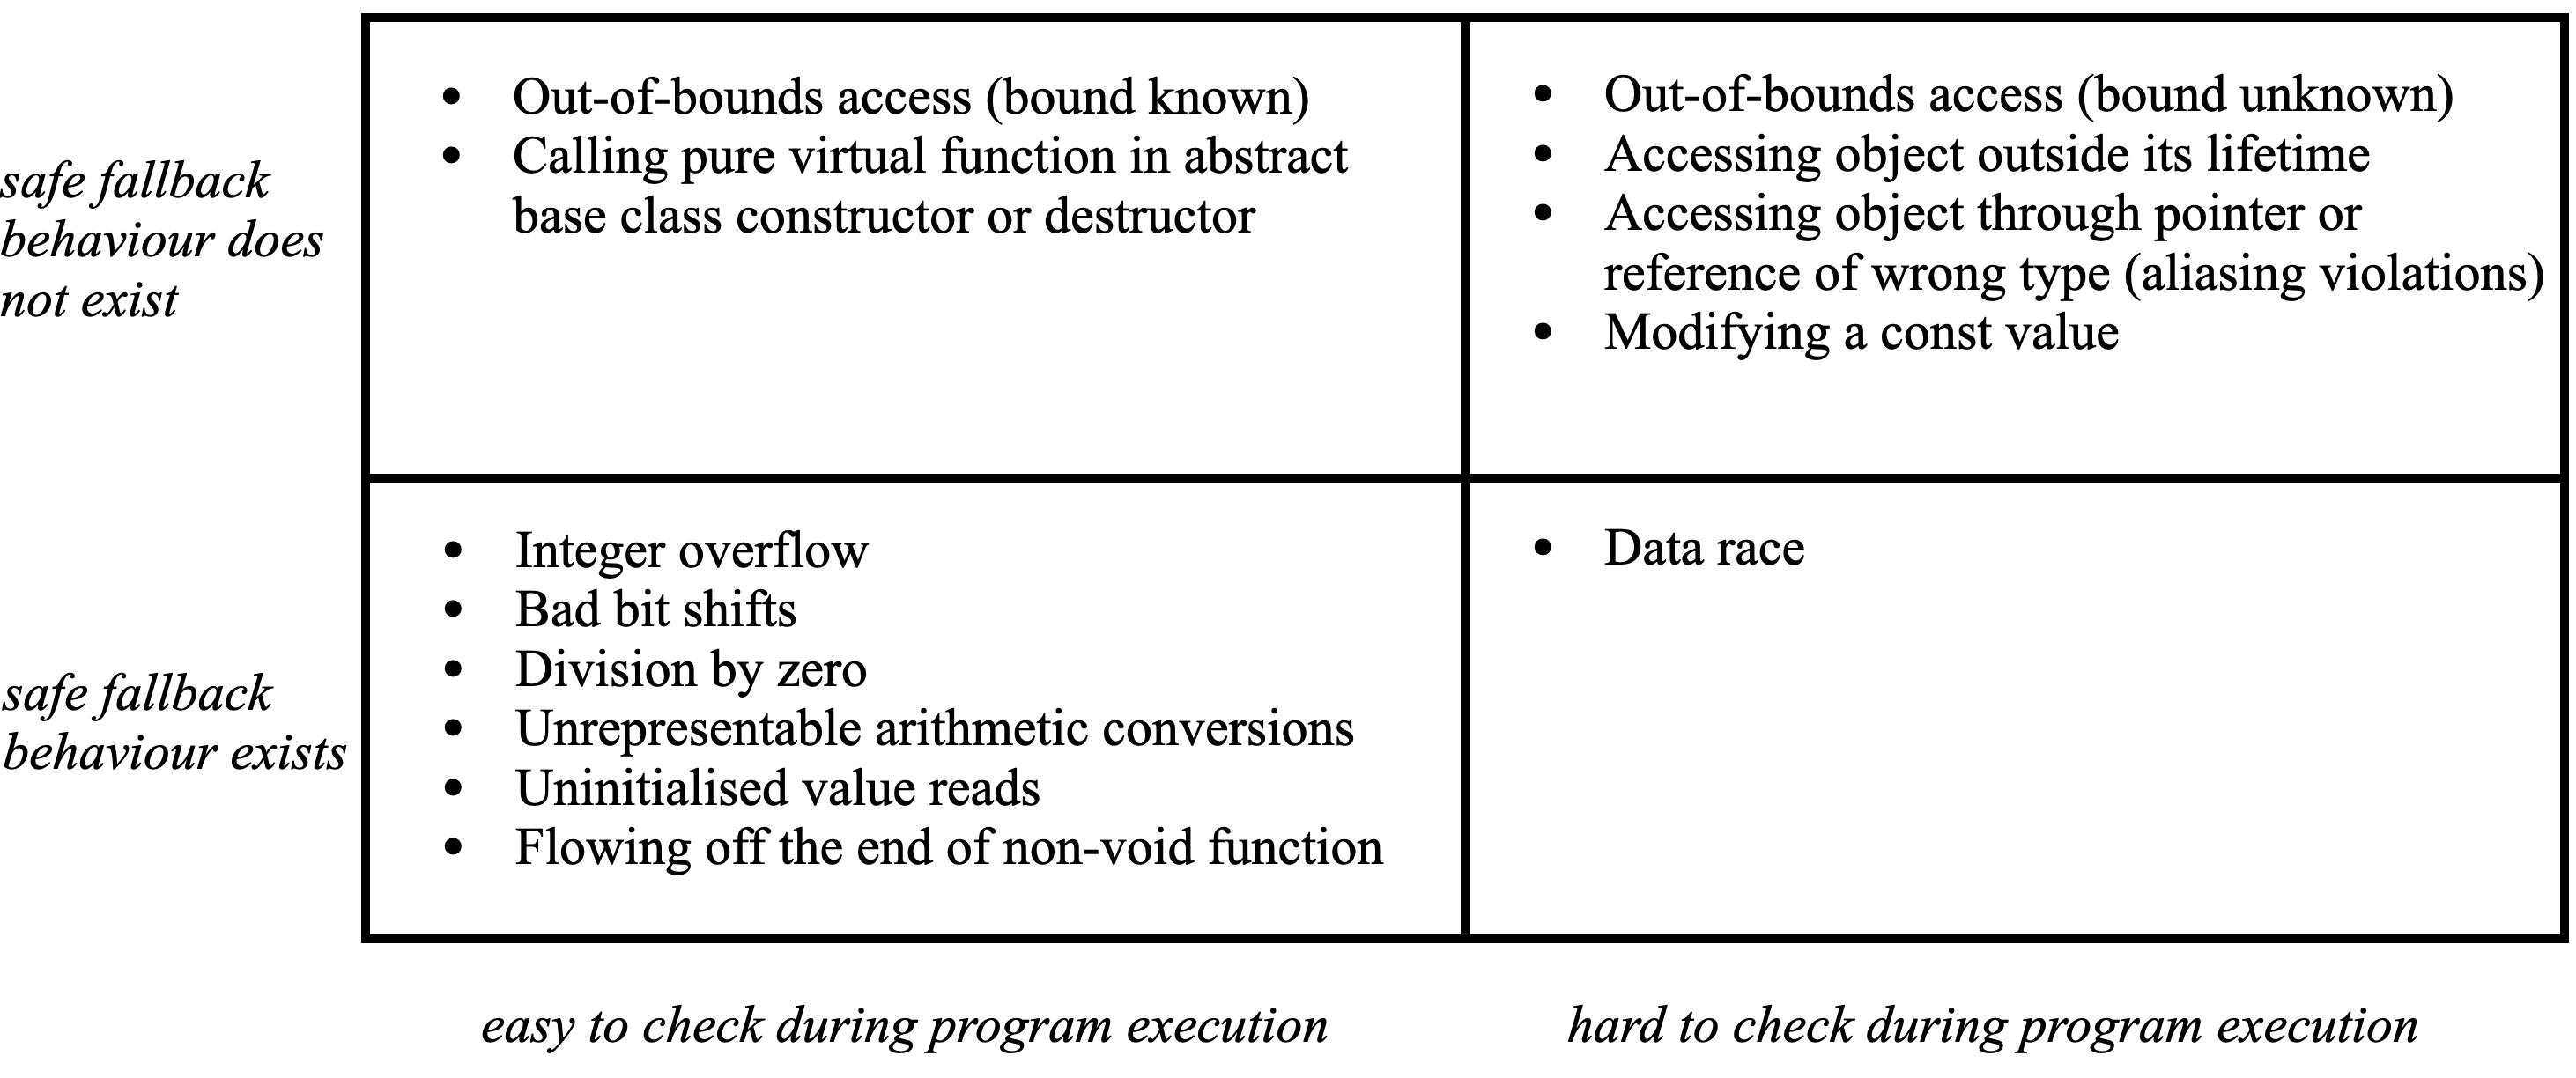
\includegraphics[scale=0.315]{images/p3100_quadrants.png}
\end{center}
\caption{Categories of undefined behaviour that can be respecified in terms of implicit contract violations}
\label{fig_quadrants}
\end{figure}
%~~~~~~~~~~~~~~~~~~~~~~~~~~~~~~~~~~~~~~~~~~~~~~~~~~~~~~~~~~~~~~~~~~~

Occurrences of undefined behaviour for which we \emph{can} define safe fallback behaviour include integer overflow, bad bit shifts, division by zero, and unrepresentable arithmetic conversions. For example, for signed integer overflow, a safe fallback behaviour is that the result of the addition will be some valid number. We could additionally specify the value of this number, for example, by specifying that signed integer overflow wraps or saturates, but to remove the undefined behaviour it is entirely sufficient to say that it will be an unspecified but valid value. Using this number in a calculation will most likely be incorrect (i.e. a bug), but it will no longer be undefined.

We can thus specify that each signed integer addition in the program behaves as-if the compiler had wrapped it into an inline function with the following precondition assertions:
\begin{codeblock}
int operator+(int a, int b)
pre ((b >= 0 && a <= INT_MAX - b) || (b < 0 && a >= INT_MIN - b));
\end{codeblock}
and that the value returned by this notional function is the sum of the two integers, or, if the operation overflows, some unspecified but valid integer. Thus, we redefine the behaviour of an operation that today has undefined behaviour, but has a reasonable safe fallback behaviour, to be \emph{that safe fallback behaviour}, guarded by the appropriate implicit contract assertions. We have thus simultaneously removed the undefined behaviour and introduced the necessary correctness checks to detect bugs due to overflow.

Note that all existing strategies for handling signed integer overflow in C++ today map exactly to one of the possible five contract evaluation semantics (the four proposed in \cite{P2900R8} plus the \emph{assume} semantic; see Section~\ref{assume}). Such strategies include:
\begin{itemize}
\item The GCC compiler option \tcode{-ftrapv}, which aborts the program on signed integer overflow, is a conforming implementation of the \emph{quick_enforce} semantic;
\item A sanitiser which detects signed integer overflow and prints a diagnostic is a conforming
implementation of the \emph{enforce} or \emph{observe} semantic (depending on whether the
process is terminated or execution continues after printing the diagnostic);
\item The GCC compiler option \tcode{-fwrapv}, which implements signed integer addition using wrap around using twos-complement representation, is a conforming implementation of the \emph{ignore} semantic, which silently executes the safe fallback behaviour;
\item The default behaviour in C++ today, which is to assume that signed integer addition can never overflow, and optimise based on this assumption when the appropriate optimisation flags are selected by the user, is a conforming implementation of the \emph{assume} semantic.
\end{itemize}

Now, let us consider an occurrence of undefined behaviour for which \emph{no} safe fallback behaviour can be reasonably defined. One example is out-of-bounds access into a raw array. What should such access return? It could return a default-constructed value of the element type, but the type may be not default-constructible. It could return an indeterminate value, similar to an uninitialised variable, but that would not improve the situation very significantly. The answer is that it should not return at all; there should be no circumstances in which control flow continues past a violation of such an implicit contract assertion. Given that it might not always be feasible to actually detect such a violation (e.g., if the bound of the array is not statically known), this leaves three out of five contract evaluation semantics as viable options:
\begin{itemize}
\item Implementations that diagnose violations of the implicit contract assertion during program execution (e.g., AddressSanitizer) can implement the \emph{enforce} or \emph{quick_enforce} semantics;
\item The default behaviour in C++ today, which is to assume that a violation can never happen, and optimise based on that assumption, is a conforming implementation of the \emph{assume} semantic.
\end{itemize}
We propose to define such operations that have no reasonable defined behaviour in case of a violation of their implicit contract  as \emph{non-ignorable implicit contract assertions}. A non-ignorable implicit contract assertion cannot be evaluated with the \emph{ignore} or \emph{observe} semantic, as there is no possible behaviour for the program for these semantics; the only possible options are to enforce or to assume that such behaviour can never occur.
% TD: the term "non-ignorable" is a bit misleading because it suggests that the assertion MUST be checked, which is
% often not possible (e.g., dangling pointers/preferences). In reality, the assertion may be enforced or assumed, but not
% ignored or observed (because there is no possible defined behaviour for the error path). Can you think of a better English
% term to express this concept?

\subsection{UB that is easy vs. difficult to diagnose during program execution}
\label{easy}

The other axis in Figure \ref{fig_quadrants} that is useful for classifying occurrences of undefined behaviour is how \emph{easy} or \emph{difficult} it would be to check for violations of the implicit contract of the affected operation. By \emph{easy} we mean an implicit contract assertion for which we can expect that a regular C++ compiler will be able to lay down runtime checks without major implementation difficulties.

An example of a non-ignorable implicit contract assertion that is \emph{easy} to check is out-of-bounds access into a raw array if the bound of the array is known at compile time; examples of ignorable implicit contract assertions with this property are integer overflow, bad bit shifts, division by zero, and unrepresentable arithmetic conversions, as well as uninitialised value reads, flowing off the end of a non-\tcode{void} function, and calling a pure virtual function in the constructor or destructor of an abstract base class.

Note that easy does not necessarily mean computationally cheap. A bounds check on array access can be insignificant in many cases; on the other hand, mitigating all occurrences of signed integer overflow can have an unacceptable performance impact for numerically heavy applications. However, in the framework of \cite{P2900R8}, the semantic of each evaluation of a contract assertion is implementation-defined and in principle independent of the semantic of any other evaluation. A conforming implementation can therefore offer separate compiler flags to turn on bounds checks and to turn on defined behaviour for signed integer overflows, respectively. This is by and large already existing practice; our proposal merely formalises this existing practice by phrasing it in terms of contract evaluation semantics, and adds extra options such as calling the contract-violation handler (see Section~\ref{handler}).

Examples of implicit contract assertions that are \emph{difficult} to check are most memory safety issues such as accessing an object outside its lifetime, accessing an object through a pointer or reference of the wrong type, and out-of-bounds access into a raw array if the bound of the array is \emph{not} known at compile time; as well as data races. By \emph{difficult} we mean that a regular C++ compiler probably will \emph{not} have the means to lay down the appropriate runtime checks, as doing so would require extensive instrumentation. Offering \emph{checked} semantics for such implicit contract assertions would therefore most typically only be offered by specialised implementations of C++ such as sanitisers (AddressSanitizer, ThreadSanitizer, etc.); our proposal would allow to reason about the semantics of such tools within the C++ Standard, and hook them into the contract-violation handler (see Section~\ref{sanitisers}).

\subsection{Explicit vs. implicit UB}

In addition to \emph{explicit} undefined behaviour, i.e. operations for which the C++ Standard explicitly states that the behaviour is undefined, there is also \emph{implicit} undefined behaviour, which occurs when the C++ Standard does not say anything at all about the runtime semantics of a particular operation.

This proposal is focused on explicit undefined behaviour, because we can specify concrete implicit contract assertions for such operations. However, we do not prevent an implementation from treating implicit undefined behaviour as a contract violation as well, if it is capable of detecting such undefined behaviour during program evaluation.

\section{Adding the missing pieces}

\subsection{The \emph{assume} semantic}
\label{assume}

We already mentioned the fifth contract evaluation semantic, \emph{assume}, in previous sections. While this semantic is not included\footnote{One of the reasons why SG21 decided to not include the \emph{assume} semantic in the first version of the proposed Contracts facility is that it has the potential to introduce undefined behaviour to an otherwise correct program via a buggy contract predicate. The presence of the \emph{assume} semantic in the C++2a Contracts proposal \cite{P0542R5} was controversial at the time and contributed to that proposal being removed from the C++20 Working Draft. An assumption facility was nevertheless seen as an important feature, and was subsequently added to C++ separately from the Contracts facility in the form of the \tcode{[[assume]]} attribute (see \cite{P1774R8}).}  in the set of semantics proposed in \cite{P2900R8}, it is an important piece of the puzzle for two reasons.

The first reason is that there are occurrences of undefined behaviour --- or, with our proposal, implicit contract assertions --- that we cannot expect every implementation of C++ to be able to check at runtime. Some of these occurrences will be operations for which there is no safe fallback behaviour --- in other words, there is no well-defined behaviour that these operations could possibly have if control flow continues past violations of their implicit preconditions. For such operations, if the compiler cannot lay down checks that can be used to \emph{enforce} the preconditions, the only other option is to compile the program with the \emph{assumption} that the check will never fail, so no instructions for this case need to be emitted by the compiler. This is the status quo today for undefined behaviour in the top right quadrant of Figure~\ref{fig_quadrants}, for example undefined behaviour due to accessing an object outside its lifetime.

The second reason is that even for implicit contract assertions that do have a safe fallback behaviour --- with our proposal, this is the behaviour that will be executed when the semantic is \emph{ignore} --- such fallback behaviour might lead to measurable performance degradations. This creates a problem for applications that care first and foremost about performance, and less about safety and security, such as high-performance numerical simulations and low-latency signal processing. Such applications must have an escape hatch that allows them to avoid degradations and preserve today's behaviour, in which the affected implicit contract assertions are \emph{assumed} rather than \emph{ignored}, with the consequence that contract violations may lead to core undefined behaviour.

For uninitialised reads, \cite{P2795R5} offers such an escape hatch in the form of the new attribute \tcode{[[indeterminate]]}, which disables the safety guardrail and restores the C++23 behaviour. However, offering such an explicit, syntactic escape hatch for every possible case of undefined behaviour does not scale; it would make the language unnecessarily complex, and in some cases, would even not be possible --- how would we annotate, for example, an expression containing signed integer addition, and would we want to do that throughout our entire numerics library? 

Our approach is therefore to offer a generic escape hatch in the form of the \emph{assume} semantic. This semantic can be selected by the user for a particular kind of implicit contract assertions, for example to squeeze maximum performance out of their numeric operations, while the other four semantics (none of which leave any room for undefined behaviour) can be used for other kinds of implicit contract assertions, for example to enable checks that guard against flowing off the end of non-\tcode{void}-returning functions. This framework enables the expert user to select precisely which tradeoffs between safety and performance are most appropriate for their use case; for the average user, implementations can offer reasonable defaults.

\subsection{The library API}
\label{lib}

Re-specifying undefined and erroneous behaviour as a contract violation as proposed here means that, if any of the introduced implicit contract assertions is determined to be violated during program execution, and the selected evaluation semantic is \emph{observe} or \emph{enforce}, the contract-violation handler will be called. In order to accommodate implicit contract assertions in the associated library API for contract-violation handling, we need to make some minor adjustments to \cite{P2900R8}.

We propose to add a new enum value \tcode{implicit} to the enum \tcode{assertion_kind}. This value will be returned from the \tcode{kind()} member function of the \tcode{contract_violation} object passed into the handler when the contract violation that caused the call to the handler resulted from an implicit rather than an explicit contract assertion. We chose the numeric value \tcode{0} for the new enum value to emphasise that it does not correspond to any kind of explicit contract assertion (i.e. an assertion that the user wrote).

We further propose that the value returned by \tcode{detection_mode()} for violations of implicit contract assertions be unspecified. This choice gives implementations freedom to specify detection modes that are best suited to express the mitigation strategies they employ, and to inform the user of the strategy used to detect a particular implicit contract violation. 

We do not propose any changes to the specification of \tcode{comment()} and \tcode{location()}. \cite{P2900R8} non-normatively recommends that these functions return a textual representation of the expression that triggered the contract violation and the source location of the contract violation, respectively. The same is in principle possible for violations of implicit contract assertions. However, generating a textual representation for every possible expression that could lead to diagnosable
undefined behaviour is likely to cause an unacceptable amount of code bloat. It is therefore equally conforming to instead generate some other string that may help the user identify the problem, such as the diagnostic message already printed by existing sanitisers. It is further conforming to simply return an empty string and a default-constructed source location if no information is available, or if the information is not programmatically accessible in the contract-violation handler (for example,
because it located in a separate debug information file). 

\section{Discussion}

\subsection{Contracts provide a framework for safety}

One benefit of adopting the framework of implicit contract assertions as proposed here for C++ is that it provides users, vendors of compilers and tools, as well as the C++ Standard committee with the vocabulary needed to reason about and  to specify different options for the detection and mitigation of undefined behaviour.

In particular, once we re-specify undefined behaviour in terms of implicit contract assertions, the \cite{P2900R8} framework specifies that any evaluation of such an assertion can have any evaluation semantic, and that the choice of semantic is implementation-defined, meaning that implementations are expected to document which semantics they support for which implicit contract assertions, and which selection mechanism they offer.

For example, a compiler that adds checks for out-of-bounds access no longer has to describe such checks as a vendor extension; it can simply document that it offers checked contract semantics for accessing an array. A user who wishes to enable such checks can more easily find tools that offer them. Further, coding guidelines can place restrictions on which semantics are permitted for which kinds of implicit contract assertions. For example, in a safety-critical context, a set of coding guidelines may prescribe that \emph{assume} semantics may not be used for certain kinds of implicit contract assertions, thus preventing the usage of toolchains and compiler options that could lead to the program exhibiting that particular kind of undefined behaviour.

Finally, re-specifying undefined behaviour in terms of implicit contract assertions would be a visible step by the C++ committee towards more safety in C++. While such re-specification in itself does not make any code safer unless compilers and tools actually offer ways to perform the additional runtime checks, it would make such efforts more visible and explicit because they would be happening within a unified Standard framework.

% TD: I am struggling to properly explain the grand vision here... it's all in my head, and I can explain it verbally (as I did in St. Louis),  but I'm too tired right now to translate it into written English :(
	
\subsection{Contracts provide a program-wide handler}
\label{handler}

Another benefit of the approach proposed here is that any compiler and tool that adds checks to detect and mitigate undefined behaviour during program execution could hook into the program-wide contract-violation handler defined by \cite{P2900R8}. This would allow the user to treat all possible defects that are detected during program execution in one place.

TODO ADD REASONS WHY THIS IS GOOD
% TD: Josh, can you elaborate on why this is a great idea? It's your idea, isn't it? A couple more paragraphs would be great but I ran out of steam here :(

\subsection{Contracts provide better integration for sanitisers}
\label{sanitisers}

The ability to interface with the Contracts machinery and the contract-violation handler applies not only to C++ compilers, but also extends to sanitisers and other tools, which might be able to offer checked semantics for a much wider range of implicit contract assertions.

The integration between such tools and user code today is poor. For example, all clang sanitisers have a callback \tcode{__sanitizer_set_death_callback}, but this callback takes no arguments. It can be used to inform the user that the process is about to terminate, but it does not provide an API to programmatically query what happened or where. ASan has a slightly more sophisticated callback \tcode{__asan_set_error_report_callback} which takes a single argument of type \tcode{const char*}. This argument provides a string that contains the generated error report.

With our proposal, all these tools can instead hook into the API provided in \cite{P2900R8} (with slight modifications as proposed in Section~\ref{lib}). This API provides not only a user callback in the form of a global replaceable contract-violation handler, but also programmatically accessible information about the defect via the  \mbox{\tcode{contract_violation}} object passed into the contract-violation handler. This more comprehensive API can serve as a uniform standard callback mechanism for sanitisers and other tools.

Note that supporting this API is entirely optional for existing sanitisers. \cite{P2900R8} specifies that the behaviour of the default contract-violation handler is implementation-defined and an implementation does not have to offer the option of installing a user-defined contract-violation handler; therefore, existing sanitisers are already conforming. Any given sanitiser can be said to apply the \tcode{enforce} evaluation semantic (without a replaceable contract-violation handler) to those kinds of undefined behaviour that it diagnoses, and the \tcode{assume} evaluation semantic to the remaining kinds.

\section{Proposal summary}
Below we provide an informal summary of the proposed changes, which are on top of those proposed in \cite{P2900R8}. Formal wording can be added after the design direction in this paper has been confirmed by the relevant study groups.

\begin{itemize}
\item Add the notion of \emph{explicit} contract assertion for a contract assertion specified by the user, which includes all three kinds of contract assertions in \cite{P2900R8} --- \tcode{pre}, \tcode{post}, and \tcode{contract_assert}.
\item Add a fifth contract evaluation semantic, the \emph{assume} semantic, to the four semantics in \cite{P2900R8}. The  \emph{assume} semantic is an unchecked semantic, i.e. it does not attempt to determine the value of the predicate. If the predicate would not evaluate to \tcode{true} at the point of evaluation of the contract assertion, the behaviour is undefined.
\item Add the notion of an \emph{implicit} contract assertion, that is, a contract assertion implicitly generated around a certain language construct by the implementation rather than specified by the user with \tcode{pre}, \tcode{post}, or \tcode{contract_assert}.
\item Add a note that implicit contract assertions can be evaluated with any of the five contract evaluation semantics, just like explicit contract assertions.
\item Remove the notion of \emph{erroneous behaviour}, replace it with ``violation of an implicit contract assertion'', and transform affected specifications as follows:
\begin{itemize}
\item Replace the specification that reading an erroneous value is erroneous behaviour with the specification that reading a value has an implicit precondition that the value is not erroneous;
\item ...
\end{itemize}
\item Transform occurrences of undefined behaviour for which a safe fallback behaviour can be specified to instead be phrased in terms of implicit contract assertions, for example:
\begin{itemize}
\item Change signed integer overflow/underflow from being undefined behaviour to producing an unspecified value; add to the specification of the the associated signed integer operations an implicit precondition that no overflow/underflow will occur;
\item Change shifting by equal or greater than the bit-width of a type from being undefined behaviour to producing an unspecified value; add to the specification of shift operations an implicit precondition that the right operand is smaller than the bit-width of the left operand;
\item Change flowing off the end of a non-\tcode{void} function from being undefined behaviour to returning an erroneous value;
\item ...
\end{itemize}
\item Add the notion of a \emph{non-ignorable} implicit contract assertion, that is, an implicit contract assertion that cannot be evaluated with the \emph{ignore} or \emph{observe} semantics;
\item Transform occurrences of undefined behaviour for which no safe fallback behaviour can be specified to instead be phrased in terms of non-ignorable contract assertions, for example:
\begin{itemize}
\item Replace the specification that accessing an object outside of its lifetime is undefined behaviour with the specification that accessing an object has a non-ignorable implicit precondition that the object is within its lifetime;
\item Replace the specification that attempting to modify a \tcode{const} object is undefined behaviour with the specification that any modification of an object has a non-ignorable implicit precondition that the object is not \tcode{const};
\item Replace the specification that incrementing a pointer beyond one past the end of an array is undefined behaviour with the specification that incrementing a pointer has a non-ignorable implicit precondition that the pointer is not beyond one past the end of an array; 
\item ...
\end{itemize}
\item Extend \tcode{std::contracts::assertion_kind} as follows:

\phantom{~~}\tcode{enum class assertion_kind \{} \\
\phantom{~~~~}\added{\tcode{implicit = 0,}} \\
\phantom{~~~~}\tcode{pre = 1,} \\
\phantom{~~~~}\tcode{post = 2,} \\ 
\phantom{~~~~}\tcode{assert = 3} \\
\phantom{~~}\tcode{\};}

where the added enum value stands for implicit contract assertions.

\item Add a provision that \tcode{std::contracts::contract_violation::detection_mode()} returns an implementation-defined value if the violated contract assertion was an implicit contract assertion.
\end{itemize}

%\section*{Document history}

%\begin{itemize}
%\item \textbf{R0}, 2023-03-08: Initial version.
%\item \textbf{R1}, 20XX-XX-XX: ??
%\end{itemize}

%\section*{Acknowledgements}

%nothing here yet

%%%%%%%%%%%%%%%%%%%%%%%%%%%%%%%%%%%%%%%%%%%%%

% Remove ToC entry for bibliography
\renewcommand{\addcontentsline}[3]{}% Make \addcontentsline a no-op to disable auto ToC entry

%\renewcommand{\bibname}{References}  % custom name for bibliography
\bibliographystyle{abstract}
\bibliography{ref}

%%%%%%%%%%%%%%%%%%%%%%%%%%%%%%%%%%%%%%%%%%%%%

\end{document}

